% ══════════════════════════════════════════════════════════════════════
% EMPIRICAL RESULTS — AGENT × TENANT EVALUATION
% Input this file inside \section{Experiments}, after \subsection{Experimental Setup}
% ══════════════════════════════════════════════════════════════════════

\subsection{Experimental Setup}
\label{sec:exp-setup}
We instantiate the three scenario families from Section~\ref{sec:scenarios} as concrete tenants (Bertrand \& Co., University of Cambford, and ZAI Intelligence) and evaluate \textcolor{blue}{four} agent configurations that span a spectrum from minimal reactive reasoning to deliberative planning; the precise model and prompt assignments are listed in Section~\ref{sec:agent-configs} and Table~\ref{tab:agent_configs}. The automated judge is GPT-4o, issuing one call per gold assertion to check satisfaction plus two calls per case for tool-search relevance and response-citation quality. Each agent is evaluated on all 525 cases (162 per small tenant, 201 for ZAI) covering the three query types defined in Section~\ref{sec:method_evaldataset}. We record both judge-based quality metrics and deterministic operational diagnostics---token usage, tool-call count, and retrieval volume---to distinguish capability failures from operational inefficiency.

\subsubsection{Agent Configurations}
\label{sec:agent-configs}
We evaluate \textcolor{blue}{four} agent configurations whose designs span a spectrum from minimal reactive reasoning to deliberative multi-step planning. All \textcolor{blue}{four} share the same embedding model (\texttt{text-embedding-ada-002}) and use GPT-4o-family models via Azure OpenAI\textcolor{blue}{: \textsc{ReAct-v1} and \textsc{ReAct-v2} use GPT-4o, while \textsc{ReAct-v3} and \textsc{Researcher} use GPT-4o-mini. This design decouples three axes---architecture (ReAct vs.\ plan-and-execute), prompt engineering (verbose vs.\ concise), and model size (GPT-4o vs.\ GPT-4o-mini)---so that pairwise comparisons can attribute gains to individual factors rather than to their confound.}

\begin{table}[h]
\centering
\caption{Configuration summary for the \textcolor{blue}{four} evaluated agents.
``Planning model'' refers to the LLM used for the optional pre-execution planning step; for \textsc{Researcher}, the same model is used for both planning and execution.
Prompt size is the approximate system-prompt token count. Avg.\ tool calls is the empirical mean across all evaluation cases.}
\label{tab:agent_configs}
\small
\begin{tabular}{p{0.13\linewidth}p{0.15\linewidth}p{0.14\linewidth}p{0.15\linewidth}p{0.13\linewidth}p{0.12\linewidth}}
\toprule
\textbf{Agent} & \textbf{Architecture} & \textbf{Model} & \textbf{Planning Model} & \textbf{Prompt Size} & \textbf{Avg.\ Tools} \\
\midrule
\textsc{ReAct-v1}   & ReAct             & GPT-4o      & ---               & $\sim$3k tok   & 1.70 \\
\textsc{ReAct-v2}   & ReAct             & GPT-4o      & ---               & $\sim$1.5k tok & 1.70 \\
\textcolor{blue}{\textsc{ReAct-v3}}   & \textcolor{blue}{ReAct}             & \textcolor{blue}{GPT-4o-mini} & \textcolor{blue}{---}               & \textcolor{blue}{$\sim$3k tok}   & \textcolor{blue}{1.23} \\
\textsc{Researcher}  & Plan\,+\,Execute  & GPT-4o-mini & GPT-4o-mini       & $\sim$3k tok   & 4.85 \\
\bottomrule
\end{tabular}
\end{table}

\textsc{ReAct-v1} implements a standard ReAct loop~\cite{yao2022react} with a verbose system prompt ($\sim$3{,}000 tokens) containing eight fully worked \textsc{Thought}$\to$\textsc{Tool} examples covering people resolution, pronoun-to-ID disambiguation, multi-query decomposition, and citation formatting. Section~\ref{sec:prompt-analysis} analyses which of these worked demonstrations drive the observed performance gap against \textsc{ReAct-v2}.

\textsc{ReAct-v2} shares the same single-pass ReAct loop but condenses the system prompt to $\sim$1{,}500 tokens across five terse bullet-style examples. The instructions cover the same topics, but replace the extended worked demonstrations with one-line directives.

\textcolor{blue}{\textsc{ReAct-v3} is a controlled ablation that shares \textsc{ReAct-v1}'s architecture and verbose prompt verbatim but swaps the backbone model from GPT-4o to GPT-4o-mini. This isolates the effect of model size at fixed architecture and prompt, which in turn lets the \textsc{ReAct-v3}\,$\leftrightarrow$\,\textsc{Researcher} comparison isolate the planning-stage effect at fixed model.}

\textsc{Researcher} instantiates the plan-and-execute strategy introduced in Section~\ref{sec:method_runtime}: GPT-4o-mini first produces a structured research plan, then the same model executes that plan step by step using the full tool set. The planning prompt explicitly requires four capabilities---(i)~multi-hop decomposition into dependency chains, (ii)~correlated search across emails, chats, meetings, and files, (iii)~mandatory name-to-ID resolution via \texttt{search\_people} before any content search, and (iv)~step-by-step ordering so that the output of each step feeds the next---and instructs the planner to output only the plan, not to execute it. As a result, \textsc{Researcher} retrieves substantially more evidence per case and consumes roughly an order of magnitude more prompt tokens than the reactive agents (quantified in Section~\ref{sec:arch-analysis}). \textcolor{blue}{Section~\ref{sec:arch-analysis} also uses the \textsc{ReAct-v3} ablation to show that the bulk of \textsc{Researcher}'s aggregate advantage over \textsc{ReAct-v1} and \textsc{ReAct-v2} comes from the choice of model family rather than from the planning stage itself.}

\textcolor{blue}{Separately from the four browsing-enabled agents above, Section~\ref{sec:ablation-tool} reports a \textsc{Retrieval} configuration that serves as a tool-ablation reference: it shares the same GPT-4o-mini backbone and index but is restricted to a single \texttt{search\_\{email,chat,meeting,file\}} call per case and cannot invoke \texttt{read\_file} (full-body reader) or \texttt{search\_in\_file} (exact-term scan). It is not included in the main results table; its purpose is solely to isolate the contribution of full-content browsing on top of snippet retrieval.}

\subsubsection{Evaluation Metrics}
\label{sec:eval-metrics}
Our experiments instantiate the configurable harness (Section~\ref{sec:method_evalharness}) with GPT-4o as the judge and three judge prompts that together score correctness, retrieval quality, and citation grounding. The resulting metric configuration is:

\begin{itemize}[leftmargin=*,itemsep=2pt,topsep=4pt]
  \item \textbf{Assertion score (Assr.)}  Each gold assertion $a_i$ is presented to the judge individually; the judge returns \textsc{True}/\textsc{False} plus a brief rationale. The case score is $\text{Assr.} = |\{a_i : \text{True}\}| / |A|$.
  \item \textbf{Tool-search relevance (TS-Rel)}  A single judge call evaluates (i)~whether the selected tools were appropriate for the query, (ii)~whether the retrieved evidence was relevant, and (iii)~whether the response is grounded in the tool results rather than hallucinated. Returns a holistic score in $[0,1]$.
  \item \textbf{Response-citation quality (RC-Rel)}  A separate judge call checks (i)~whether a \texttt{\#\#~References} section exists, (ii)~whether each cited artifact ID appears in the tool-call trace (grounded) or was fabricated (hallucinated), and (iii)~whether inline citation markers appear in the response body. Returns a score in $[0,1]$.
  \item \textbf{Combined citation score (Cite)}  Equal-weight mean of TS-Rel and RC-Rel, summarising end-to-end evidence handling.
\end{itemize}

\textbf{Deterministic diagnostics} collected without LLM calls: TS-$n$ (retrieved-item count) and RC-$n$ (response citation count).

\textbf{Pass/fail rule.}  Following the two-gate criterion motivated in Section~\ref{sec:method_evalharness}, a case is marked \emph{passed} when Assr.\ $\geq 0.75$ \emph{and} RC-Rel $\geq 0.7$, i.e., both the correctness gate and the grounding gate hold simultaneously. Pass rate is the fraction of cases that satisfy both gates. \textcolor{blue}{We verified rank stability under this threshold choice by sweeping the assertion gate $\tau \in \{0.70, 0.75, 0.80, 0.90, 1.00\}$ while holding the RC-Rel gate fixed at 0.7. The agent ranking is preserved in every (agent, tenant) cell (Appendix Table~\ref{tab:threshold_sensitivity}): no cell reverses ordering across $\tau$, and pass-rate vectors are monotone non-increasing in $\tau$ as expected.}

\subsection{Main Results}
\label{sec:main-results}

\subsubsection{Overall Results}
\label{sec:overall-results}

Table~\ref{tab:results_full} reports the decomposed metrics across all \textcolor{blue}{twelve} agent--tenant combinations\textcolor{blue}{, with each pass-rate estimate augmented by a 95\% Wilson confidence interval. Paired Wilcoxon signed-rank tests between selected agent pairs on matched case IDs (reported inline below) are summarised in Appendix Table~\ref{tab:wilcoxon_full} for completeness.}

\begin{table}[h]
\centering
\caption{Per-tenant and per-agent evaluation results.
\emph{Pass}: pass rate\textcolor{blue}{\ (with 95\% Wilson CI in brackets)}. \emph{Assr.}: assertion score. \emph{TS-Rel}: tool-search relevance. \emph{TS-$n$}: mean items retrieved. \emph{RC-Rel}: response-citation relevance. \emph{RC-$n$}: mean grounded citations. \emph{Cite}: composite citation score (mean of TS-Rel and RC-Rel).
Bold marks the best per-tenant value.}
\label{tab:results_full}
\resizebox{\linewidth}{!}{%
\begin{tabular}{llccccccc}
\toprule
\textbf{Tenant} & \textbf{Agent} & \textbf{Cases} & \textbf{Pass \textcolor{blue}{[95\% CI]}} & \textbf{Assr.} & \textbf{TS-Rel} & \textbf{TS-$n$} & \textbf{RC-Rel} & \textbf{Cite} \\
\midrule
\multirow{4}{*}{Bertrand}
  & \textsc{ReAct-v1}   & 162 & 0.414 \textcolor{blue}{[.341,.491]} & \textbf{0.736} & \textbf{0.803} & 19.2 & 0.593              & 0.698              \\
  & \textsc{ReAct-v2}   & 162 & 0.259 \textcolor{blue}{[.198,.332]} & 0.729          & 0.650          & 15.8 & 0.479              & 0.565              \\
  & \textcolor{blue}{\textsc{ReAct-v3}}   & \textcolor{blue}{162} & \textcolor{blue}{0.395 [.323,.472]} & \textcolor{blue}{0.666}          & \textcolor{blue}{0.789}          & \textcolor{blue}{43.0} & \textcolor{blue}{\textbf{0.665}}     & \textcolor{blue}{\textbf{0.727}}     \\
  & \textsc{Researcher}  & 162 & \textbf{0.432} \textcolor{blue}{[.358,.509]}     & 0.625          & 0.762          & \textbf{61.1} & 0.640              & 0.701              \\
\midrule
\multirow{4}{*}{Cambford}
  & \textsc{ReAct-v1}   & 162 & 0.228 \textcolor{blue}{[.171,.299]} & 0.515          & 0.717          & 18.3 & 0.449              & 0.583              \\
  & \textsc{ReAct-v2}   & 162 & 0.222 \textcolor{blue}{[.165,.292]} & 0.489          & 0.701          & 17.0 & 0.440              & 0.571              \\
  & \textcolor{blue}{\textsc{ReAct-v3}}   & \textcolor{blue}{162} & \textcolor{blue}{0.296 [.231,.371]} & \textcolor{blue}{\textbf{0.539}} & \textcolor{blue}{\textbf{0.808}} & \textcolor{blue}{36.4} & \textcolor{blue}{\textbf{0.700}}     & \textcolor{blue}{\textbf{0.754}}     \\
  & \textsc{Researcher}  & 162 & \textbf{0.346} \textcolor{blue}{[.277,.422]}     & 0.543 & 0.793          & \textbf{61.1} & 0.684              & 0.738              \\
\midrule
\multirow{4}{*}{ZAI}
  & \textsc{ReAct-v1}   & 201 & 0.269 \textcolor{blue}{[.212,.334]} & 0.560 & 0.797          & 17.9 & 0.558              & 0.677     \\
  & \textsc{ReAct-v2}   & 201 & 0.154 \textcolor{blue}{[.111,.211]} & 0.473          & 0.717          & 13.5 & 0.493              & 0.605              \\
  & \textcolor{blue}{\textsc{ReAct-v3}}   & \textcolor{blue}{201} & \textcolor{blue}{\textbf{0.363} [.300,.432]} & \textcolor{blue}{\textbf{0.569}}          & \textcolor{blue}{\textbf{0.797}}          & \textcolor{blue}{36.6} & \textcolor{blue}{\textbf{0.740}}     & \textcolor{blue}{\textbf{0.768}}     \\
  & \textsc{Researcher}  & 201 & 0.289 \textcolor{blue}{[.230,.355]}     & 0.503          & 0.765          & \textbf{62.5} & 0.623     & 0.694              \\
\bottomrule
\end{tabular}
}
\end{table}

\begin{figure}[h]
\centering
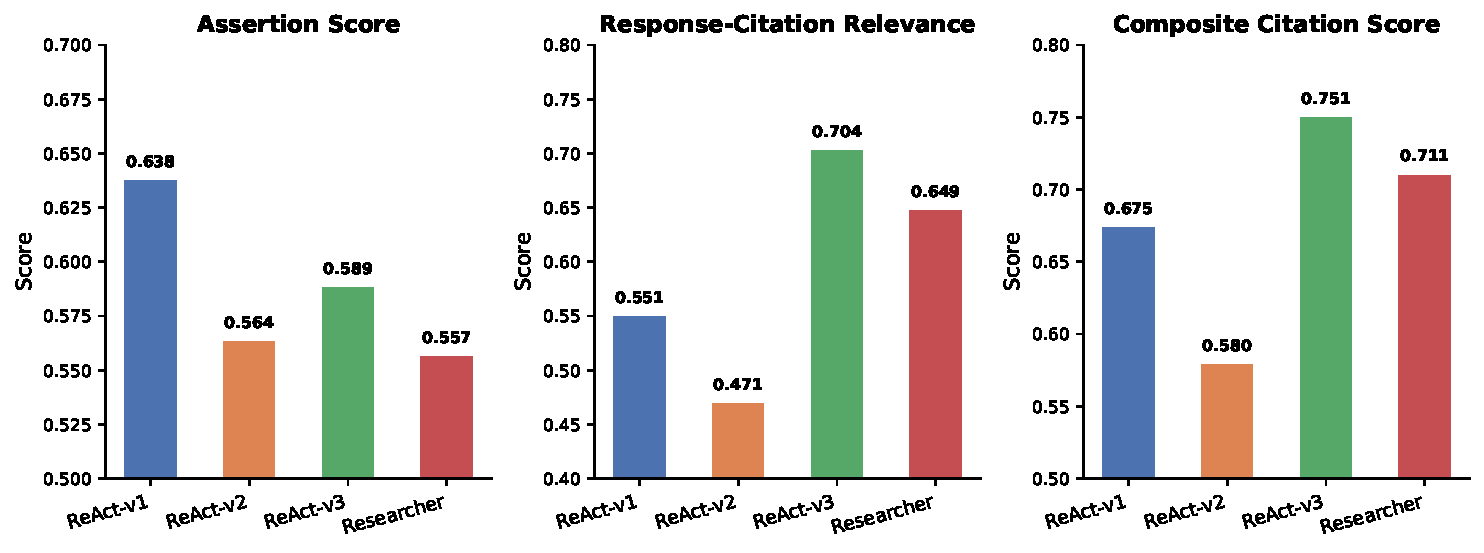
\includegraphics[width=\linewidth]{figures/aggregate_assr_rcrel.pdf}
\caption{Weighted-aggregate metrics across all tenants. \emph{Left}: assertion score---\textsc{ReAct-v1} leads (0.638). \emph{Middle}: response-citation relevance---\textsc{ReAct-v3} leads (0.704). \emph{Right}: composite citation score (mean of TS-Rel and RC-Rel)---\textsc{ReAct-v3} leads (0.751).}
\label{fig:aggregate_assr_rcrel}
\end{figure}

\subsubsection{Comparisons of the Four Methods}
\label{sec:method-comparisons}

\noindent \textcolor{blue}{The aggregate picture changes substantially once the model-size variable is held fixed. \textsc{Researcher} (0.355 pass, 95\% CI [.316,.395]) and the \textsc{ReAct-v3} ablation (0.352 pass, 95\% CI [.312,.394]) are statistically indistinguishable in aggregate, even though \textsc{ReAct-v3} uses no planning stage and less than a third of the prompt tokens (27.4k vs.\ 92.3k). \textsc{ReAct-v3} also achieves the highest composite citation score (Cite\,$=$\,0.751) and tool-search relevance (TS-Rel\,$=$\,0.798), indicating that its retrieval quality exceeds all other agents despite using fewer tool calls (1.23 vs.\ 4.85 for \textsc{Researcher}). \textsc{ReAct-v1} (GPT-4o + verbose prompt) trails at 0.323 pass but attains the best mean assertion score (0.638), while \textsc{ReAct-v2} is clearly dominated at 0.212 across all metrics. The per-tenant picture is more nuanced: \textsc{Researcher} remains best on Bertrand (0.432) and Cambford (0.346, and the only cell where the advantage over \textsc{ReAct-v1} is significant at $p{=}5.6\mathrm{e}{-3}$), but \textsc{ReAct-v3} is the single best agent on ZAI (0.363 pass, 0.740 RC-Rel, 0.768 Cite) and significantly beats \textsc{Researcher} there ($p{=}0.032$, paired Wilcoxon). \textsc{ReAct-v3} also outperforms \textsc{ReAct-v2} at fixed model on ZAI ($p{=}5.7\mathrm{e}{-8}$), isolating the benefit of the verbose prompt. These contrasts reshape the headline conclusion: rather than ``plan-and-execute wins'', the evidence supports ``plan-and-execute wins on temporally dispersed, multi-hop workloads (Cambford) but ties or loses on dense, bursty workloads (ZAI, Bertrand) once the model-family confound is removed.''}

\subsection{Ablation Studies}
\label{sec:ablations}

This section isolates the contribution of each design axis along which our agent configurations differ. We consider three orthogonal axes in turn: architecture (ReAct vs.\ plan-and-execute at fixed model), backbone model (GPT-4o vs.\ GPT-4o-mini at fixed architecture and prompt), and tool surface (snippet-only retrieval vs.\ full-content browsing).

\subsubsection{ReAct vs.\ Plan-and-Execute}
\label{sec:arch-analysis}
The primary architectural difference between \textsc{Researcher} and the two reactive agents is the separation of planning from execution described in Section~\ref{sec:agent-configs}. \textcolor{blue}{Because \textsc{Researcher} and \textsc{ReAct-v3} share the GPT-4o-mini backbone and differ only in the presence of a planning stage, the \textsc{ReAct-v3}\,$\leftrightarrow$\,\textsc{Researcher} contrast isolates the planning effect at fixed model.} The planning-stage design directly explains three empirical patterns.

First, \textsc{Researcher} retrieves 61.6 items per case versus 15--19 for the GPT-4o reactive agents (\textsc{ReAct-v3} retrieves 38.5)---a factor of $\sim$3--4$\times$. The planning prompt explicitly requires correlated search across emails, chats, meetings, and files, whereas the reactive agents only pursue additional artifact types opportunistically. This broader retrieval footprint is the primary driver of the response-citation advantage: with more retrieved artifacts available, the execution model has more material to cite, raising the grounded-citation count from 1.87 (v1) to 2.81 (\textsc{Researcher}).

\begin{figure}[h]
\centering
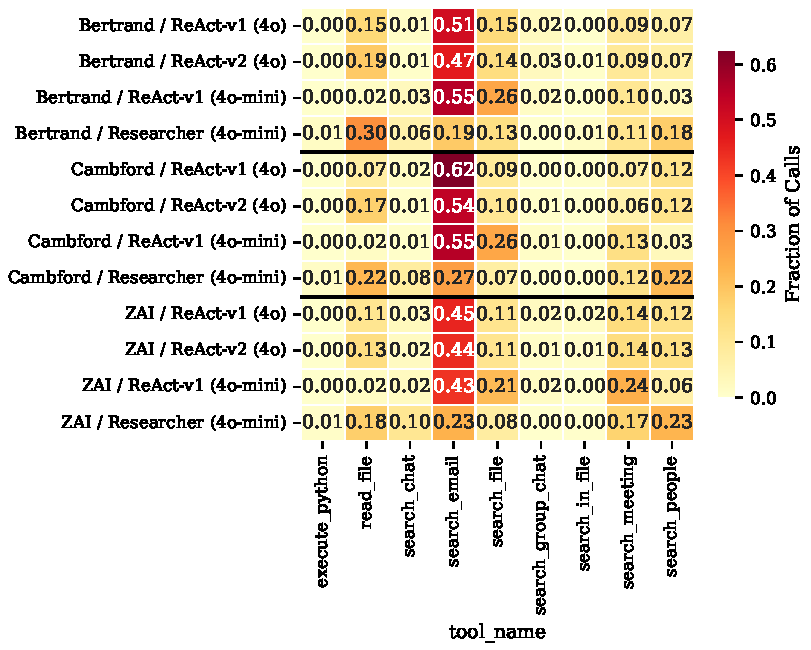
\includegraphics[width=0.85\linewidth]{figures/tool_usage_heatmap.pdf}
\caption{Tool-call distribution by agent and tenant. Rows are grouped by tenant; columns show individual tools. \textsc{Researcher} allocates calls across more tool types in every tenant, while the reactive agents concentrate on \texttt{search\_messages} and \texttt{search\_people}. Cross-tenant variation is visible: ZAI's larger corpus drives higher \texttt{read\_file} usage across all agents.}
\label{fig:tool_usage}
\end{figure}

Second, the planning stage is most beneficial when queries require temporal multi-hop reasoning. On Cambford, where cases frequently require reconstructing policy evolution across weeks of committee emails and subsequent meeting threads, \textsc{Researcher} improves pass rate by 52\% relative to \textsc{ReAct-v1} (0.346 vs.\ 0.228\textcolor{blue}{, paired Wilcoxon $p{=}5.6\mathrm{e}{-3}$}) and achieves the highest citation score in any cell (0.738). On Bertrand, where the smaller, denser organization makes most answers reachable via a single well-formed search, the pass-rate gap shrinks to 4\% (0.432 vs.\ 0.414)\textcolor{blue}{\ and is no longer significant ($p{=}0.68$)}. On ZAI, where evidence is concentrated in dense operational bursts, \textsc{ReAct-v1} closes to within 2 percentage points of \textsc{Researcher} on pass rate (0.269 vs.\ 0.289\textcolor{blue}{, $p{=}0.57$}) and substantially exceeds it on assertion score (0.560 vs.\ 0.503).

Third, despite leading on pass rate and citation, \textsc{Researcher} lags on assertion score (0.557 vs.\ 0.638 for v1). The smaller GPT-4o-mini model has lower per-call reasoning capacity than GPT-4o. The planning stage further compounds this by guiding execution toward broad retrieval at the expense of precise fact synthesis. The result is a coverage-vs.-precision trade-off: \textsc{Researcher} achieves broad retrieval coverage at the cost of per-assertion accuracy.

\subsubsection{\textcolor{blue}{Model-wise Comparison (GPT-4o vs.\ GPT-4o-mini)}}
\label{sec:ablation-model}
\textcolor{blue}{The \textsc{ReAct-v1}\,$\leftrightarrow$\,\textsc{ReAct-v3} pair holds architecture and the verbose prompt fixed while swapping the backbone from GPT-4o to GPT-4o-mini, cleanly isolating the model-family effect. Combined with the planning contrast above, this lets us decompose the aggregate \textsc{Researcher}\,$-$\,\textsc{ReAct-v1} gap into two orthogonal contributions. Holding architecture and prompt fixed and varying only model family yields per-tenant pass-rate changes of $-0.019$ / $+0.068$ / $+0.094$ on Bertrand / Cambford / ZAI respectively, i.e., GPT-4o-mini is neutral-to-better on all three tenants and strongly better on the bursty ZAI workload. Holding model fixed and adding the planning stage (\textsc{ReAct-v3}\,$\to$\,\textsc{Researcher}) yields $+0.037$ / $+0.050$ / $-0.074$: planning gives a modest boost on Bertrand and Cambford but is actively harmful on ZAI, where the planner issues extra retrieval steps that consume context budget without adding new evidence. The planner's aggregate $0.355 > 0.323$ advantage over \textsc{ReAct-v1} is therefore a composite of a real planning benefit on Cambford and a model-family effect that moves in the opposite direction on ZAI. A practitioner choosing an agent should read Table~\ref{tab:results_full} row-by-row rather than relying on the aggregate, because the correct winner depends strongly on the target tenant's temporal structure.}

\subsubsection{\textcolor{blue}{Tool-wise Ablation: Full-Content Browsing}}
\label{sec:ablation-tool}
\textcolor{blue}{The agents reported above are all granted a rich browsing surface---in addition to the four \texttt{search\_\{email,chat,meeting,file\}} endpoints that return ranked snippets, each of them can call \texttt{read\_file} to fetch the complete body of an already-identified artifact and \texttt{search\_in\_file} to perform an exact-term scan inside that body. To quantify what this full-content browsing buys, we run a tool ablation in which every other component of the runtime is held fixed and the tool surface is collapsed to snippet retrieval only. The resulting \textsc{Retrieval} configuration is defined in Section~\ref{sec:agent-configs}: it issues exactly one \texttt{search\_*} call per case against the same hybrid index, produces a grounded answer from the returned snippets, and is forbidden from invoking either \texttt{read\_file} or \texttt{search\_in\_file}. The gap between \textsc{Retrieval} and the reactive agents therefore isolates the joint contribution of (i)~iterating beyond a single retrieval, (ii)~reading the full artifact body instead of a snippet, and (iii)~using exact-term matches inside that body to disambiguate candidates.}

\begin{table}[h]
\centering
\caption{Mean tool calls per case by agent, aggregated across all three tenants.
\emph{Email/Chat/Meeting/File}: content-search endpoints returning ranked snippets.
\emph{People}: name-to-ID resolution.
\emph{Read}: full-body artifact retrieval (\texttt{read\_file}).
\emph{Search-in}: exact-term scan inside an artifact (\texttt{search\_in\_file}).
\textsc{Retrieval} is restricted to a single snippet-search call by construction.}
\label{tab:tool_usage}
\small
\begin{tabular}{lccccccc|c}
\toprule
\textbf{Agent} & \textbf{Email} & \textbf{Chat} & \textbf{Meet.} & \textbf{File} & \textbf{People} & \textbf{Read} & \textbf{Search-in} & \textbf{Total} \\
\midrule
\textsc{ReAct-v1}   & 0.81 & 0.05 & 0.17 & 0.19 & 0.18 & 0.27          & 0.01          & 1.69 \\
\textsc{ReAct-v2}   & 0.81 & 0.06 & 0.17 & 0.18 & 0.16 & 0.17          & 0.01          & 1.56 \\
\textcolor{blue}{\textsc{ReAct-v3}}   & \textcolor{blue}{0.62} & \textcolor{blue}{0.04} & \textcolor{blue}{0.20} & \textcolor{blue}{0.30} & \textcolor{blue}{0.05} & \textcolor{blue}{0.02} & \textcolor{blue}{0.00} & \textcolor{blue}{1.23} \\
\textsc{Researcher}  & 0.96 & 0.34 & 0.56 & 0.39 & \textbf{0.87} & \textbf{0.97} & 0.03          & \textbf{4.17} \\
\midrule
\textcolor{blue}{\textsc{Retrieval}}  & \textcolor{blue}{0.96} & \textcolor{blue}{0.01} & \textcolor{blue}{0.03} & \textcolor{blue}{---} & \textcolor{blue}{---} & \textcolor{blue}{---} & \textcolor{blue}{---} & \textcolor{blue}{1.00} \\
\bottomrule
\end{tabular}
\end{table}

\begin{figure}[h]
\centering
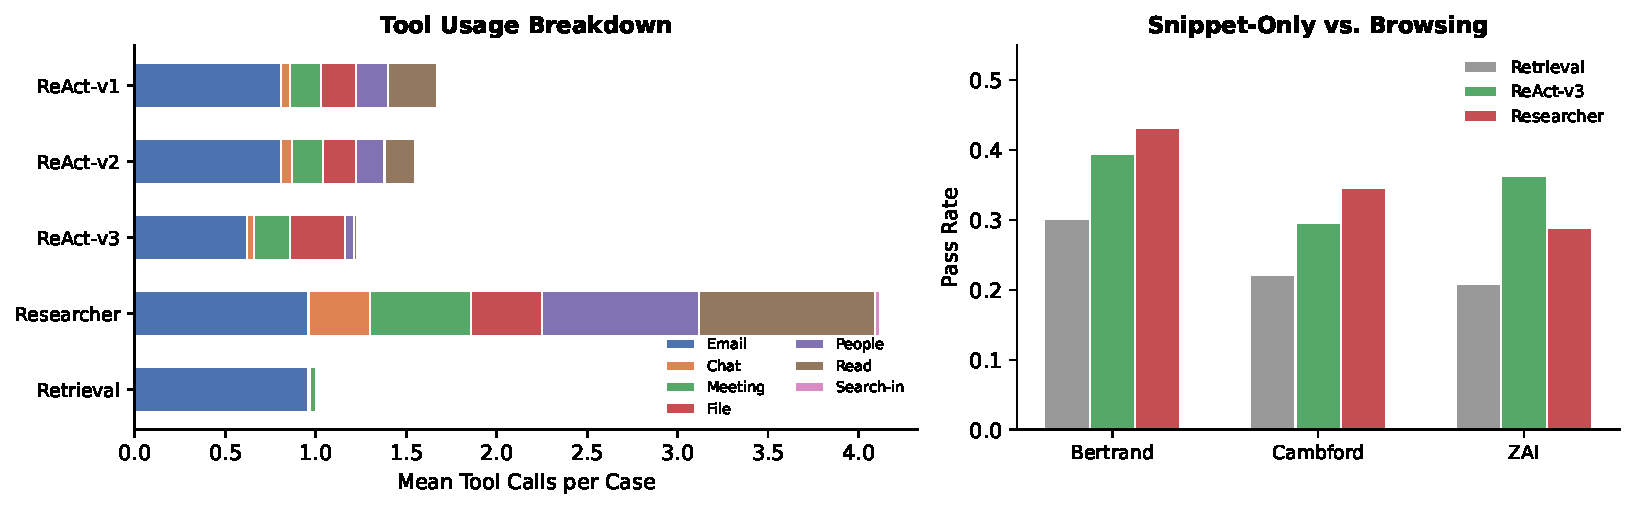
\includegraphics[width=\linewidth]{figures/tool_ablation_combined.pdf}
\caption{\emph{Left}: stacked tool-call breakdown per agent (mean calls/case across 525 cases). \textsc{Researcher} uses $4\times$ more tools than the reactive agents, dominated by \texttt{search\_people} and \texttt{read\_file}. \textsc{Retrieval} is restricted to a single snippet-search call. \emph{Right}: per-tenant pass-rate comparison between snippet-only \textsc{Retrieval} and two browsing-enabled agents. Browsing yields a consistent 9--15 point lift on Bertrand and Cambford; on ZAI, \textsc{ReAct-v3} gains 15 points while \textsc{Researcher} gains only 8.}
\label{fig:tool_ablation}
\end{figure}

\textcolor{blue}{Table~\ref{tab:tool_usage} and Figure~\ref{fig:tool_ablation} contrast tool-usage patterns and the browsing-ablation results. Three observations stand out. (1)~\emph{Tool diversity separates the planner from the reactive agents.} \textsc{Researcher} calls \texttt{search\_people} (0.87/case) and \texttt{read\_file} (0.97/case) far more than any reactive agent; its planning stage explicitly mandates name-to-ID resolution before content search. The reactive agents concentrate on \texttt{search\_email} and rarely invoke full-body reading. (2)~\emph{Snippet-only retrieval is a genuine floor, not a ceiling.} Pooled over 525 matched cases, \textsc{Retrieval} attains $24.2\%$ pass versus $35.5\%$ for \textsc{Researcher} and $35.2\%$ for \textsc{ReAct-v3}---an $11$--$12$ point absolute gap. The gap maps onto exactly the capability that \texttt{read\_file} and \texttt{search\_in\_file} unlock: retrieving a snippet suffices to cite an artifact, but reading its full body is what turns a plausible citation into a correct assertion. (3)~\emph{Browsing does not help a bad agent.} \textsc{ReAct-v2}, whose prompt does not exploit the browsing tools effectively, is statistically indistinguishable from \textsc{Retrieval} on all three tenants ($p\in\{0.35, 1.00, 0.12\}$) and even trails it on ZAI (15.4\% vs.\ 20.9\%). In other words, access to full-content browsing is necessary but not sufficient; the agent must actually use it.}

\subsection{Case Studies}
\label{sec:case-studies}

\subsubsection{Effect of Prompt Engineering}
\label{sec:prompt-analysis}
\textsc{ReAct-v1} and \textsc{ReAct-v2} share the same architecture, backbone model (GPT-4o), and tool set, yet their aggregate pass rates differ by 11 percentage points (32.3\% vs.\ 21.2\%). System-prompt verbosity is the primary driver of this gap. \textsc{ReAct-v1}'s eight fully worked examples concretely demonstrate each behavioral pattern: the agent sees a complete \textsc{Thought}$\to$\textsc{Tool}$\to$\textsc{Observation} chain for dual-term person lookup, pronoun resolution, multi-query decomposition, Python analytics, and citation formatting. \textsc{ReAct-v2}'s five bullet-style examples state the same requirements but as abstract directives rather than worked instances. The consequence is most visible in citation behavior: v2's response-citation relevance (0.471) is 8 points below v1's (0.551), suggesting that the model benefits more from seeing the correct citation format demonstrated than from being told to produce it. Tool-search relevance drops even more sharply (0.689 vs.\ 0.785), indicating that the condensed prompt also impairs the quality of the search queries themselves, not just the final formatting. The composite citation score reflects both gaps: v1's aggregate Cite (0.675) exceeds v2's (0.580) by nearly 10 points.

\subsubsection{Scenario-Level Analysis}
\label{sec:scenario-analysis}

The three tenants stress different agent capabilities, and the per-tenant results expose the conditions under which each architecture excels or fails.

\paragraph{Bertrand \& Co.\ (Legal).} Bertrand is the smallest and densest tenant (Table~\ref{tab:network_metrics}), so most entities are reachable within two hops and a single well-executed tool call frequently suffices. All four agents perform comparably on pass rate---\textsc{ReAct-v1} at 0.414, \textsc{ReAct-v3} at 0.395, and \textsc{Researcher} at 0.432---and \textsc{ReAct-v1} leads decisively on assertion score (0.736 vs.\ 0.625 for \textsc{Researcher}). \textsc{ReAct-v3} achieves the highest RC-Rel (0.665) and Cite (0.727). The planning overhead provides near-zero benefit when evidence is organizationally concentrated.

\paragraph{Univ.\ of Cambford (Education).} This tenant, designed around multi-week committee processes (Section~\ref{sec:scenarios}), is the most challenging for reactive agents: without an explicit dependency-chain plan, \textsc{ReAct-v1} achieves only 0.228 and \textsc{ReAct-v2} 0.222---barely distinguishable. \textsc{Researcher}'s planning stage raises pass rate to 0.346 and Cite to 0.738, the highest across all twelve cells. \textsc{ReAct-v3} also benefits from the GPT-4o-mini backbone here, reaching 0.296 pass and the highest RC-Rel (0.700) and Cite (0.754) on this tenant. This scenario is the clearest demonstration of when plan-and-execute provides a qualitative advantage over reactive reasoning.

\paragraph{ZAI Intelligence (Software / AI).} ZAI combines the largest scale (Table~\ref{tab:network_metrics}) with the highest chat burstiness ($B = 0.658$, Table~\ref{tab:iet_summary}), producing dense same-day clusters of engineering activity. Here the reactive agents are competitive because a well-targeted single search often retrieves several related artifacts simultaneously. \textsc{ReAct-v3} is the outright winner on ZAI (0.363 pass, 0.740 RC-Rel, 0.768 Cite), while \textsc{ReAct-v1} achieves 0.269 pass and the highest per-tenant assertion score (0.560)---substantially above \textsc{Researcher}'s 0.503. \textsc{Researcher}'s 0.289 pass rate places it below both \textsc{ReAct-v3} and \textsc{ReAct-v1}, suggesting that the planning overhead can be counterproductive when evidence is dense: the planner introduces additional, potentially irrelevant search steps that consume context budget without improving accuracy.

\begin{figure}[h]
\centering
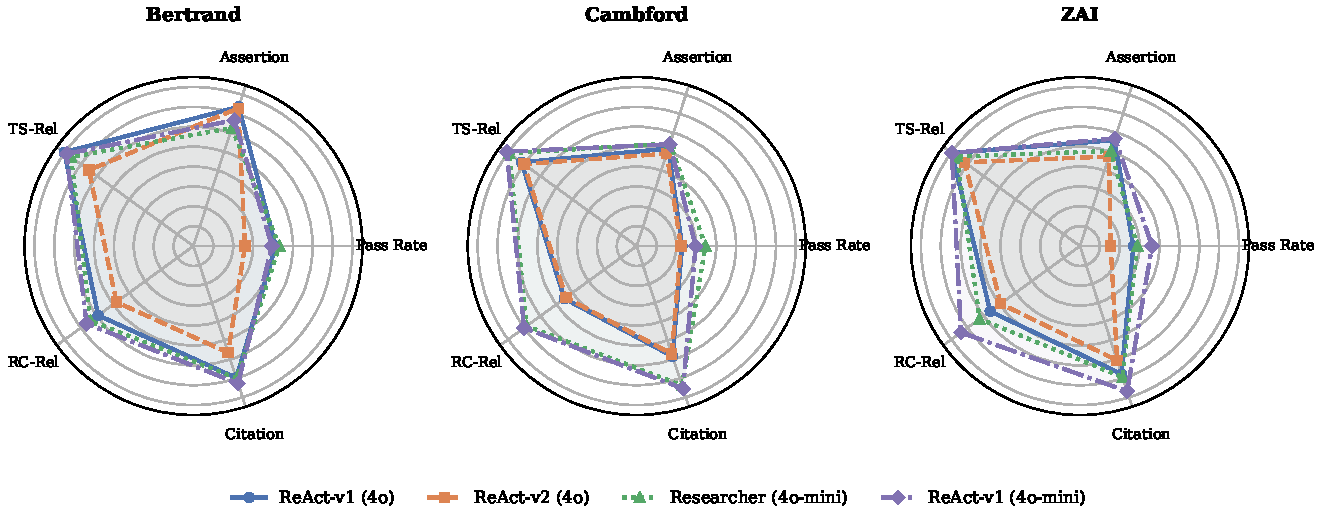
\includegraphics[width=\linewidth]{figures/agent_radar.pdf}
\caption{Per-tenant agent profiles. Each subplot shows the \textcolor{blue}{four} agents on a shared radar for one tenant. On Bertrand (dense, small) all agents overlap; on Cambford (temporal multi-hop) \textsc{Researcher}'s citation and pass-rate advantage widens; on ZAI (large, bursty) \textcolor{blue}{\textsc{ReAct-v3}} matches or exceeds the planner on assertion accuracy.}
\label{fig:agent_radar}
\end{figure}

\subsubsection{Query-Type Analysis}
\label{sec:query-type-analysis}

The evaluation set comprises the three query categories defined in Section~\ref{sec:method_evaldataset}, generated with a 40/40/20 target split. Breaking down assertion and citation metrics by query type reveals how each architecture handles increasing retrieval complexity. Query types are assigned by the generator at case-creation time and recorded in the \texttt{query\_type} field of the evaluation JSON; the reported split is derived from that field rather than from any post-hoc classification.

\begin{figure}[h]
\centering
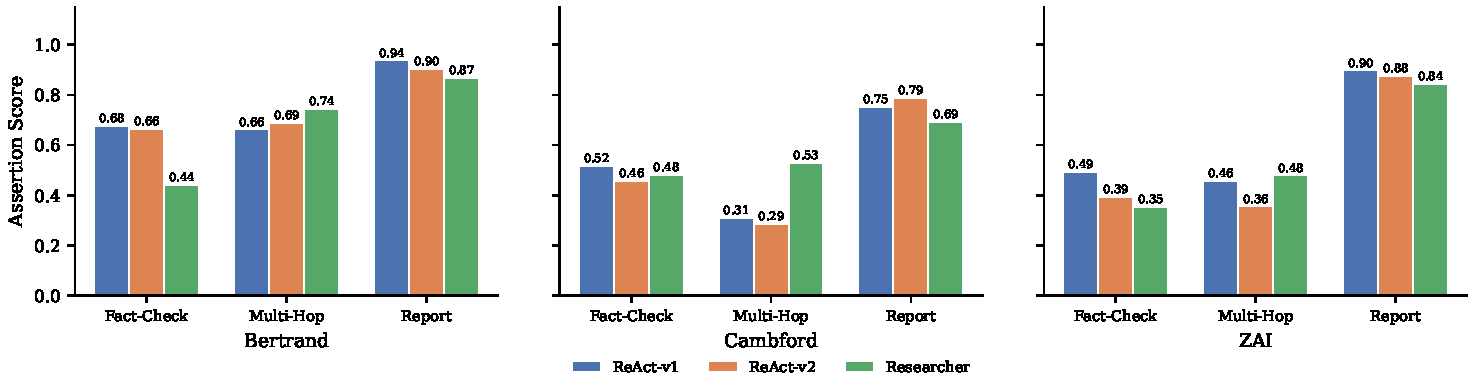
\includegraphics[width=\linewidth]{figures/assertion_by_query_type.pdf}
\caption{Mean assertion score by query type and tenant. All agents perform best on targeted artifact search queries. The gap between agents widens on multi-hop reasoning and comprehensive report queries, where \textsc{ReAct-v1}'s precision advantage is most pronounced.}
\label{fig:assertion_by_query_type}
\end{figure}

\begin{figure}[h]
\centering
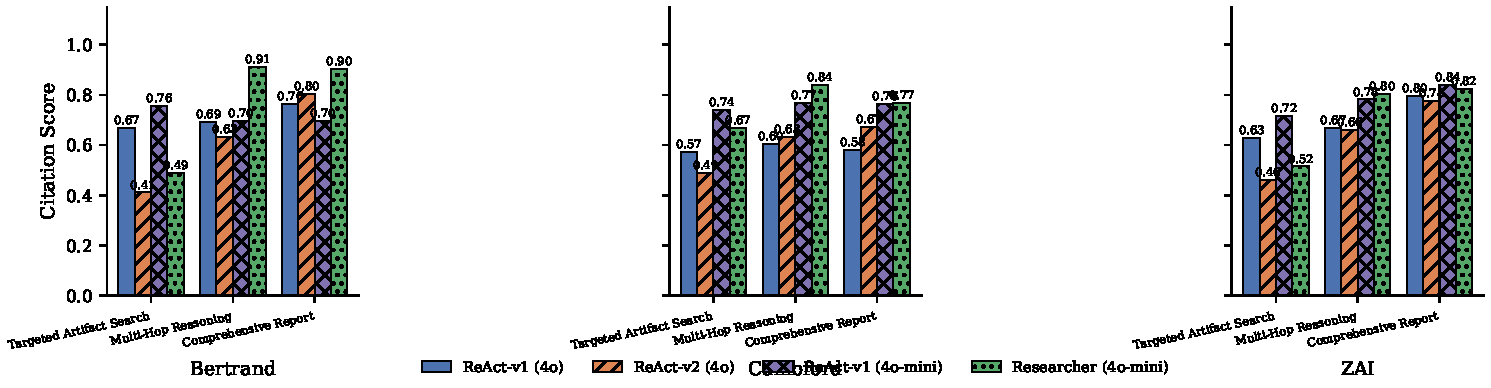
\includegraphics[width=\linewidth]{figures/citation_by_query_type.pdf}
\caption{Mean citation score by query type and tenant. \textsc{Researcher} leads on comprehensive report queries where its planning stage systematically covers multiple source types, while the reactive agents are competitive on targeted artifact search queries.}
\label{fig:citation_by_query_type}
\end{figure}

\begin{figure}[h]
\centering
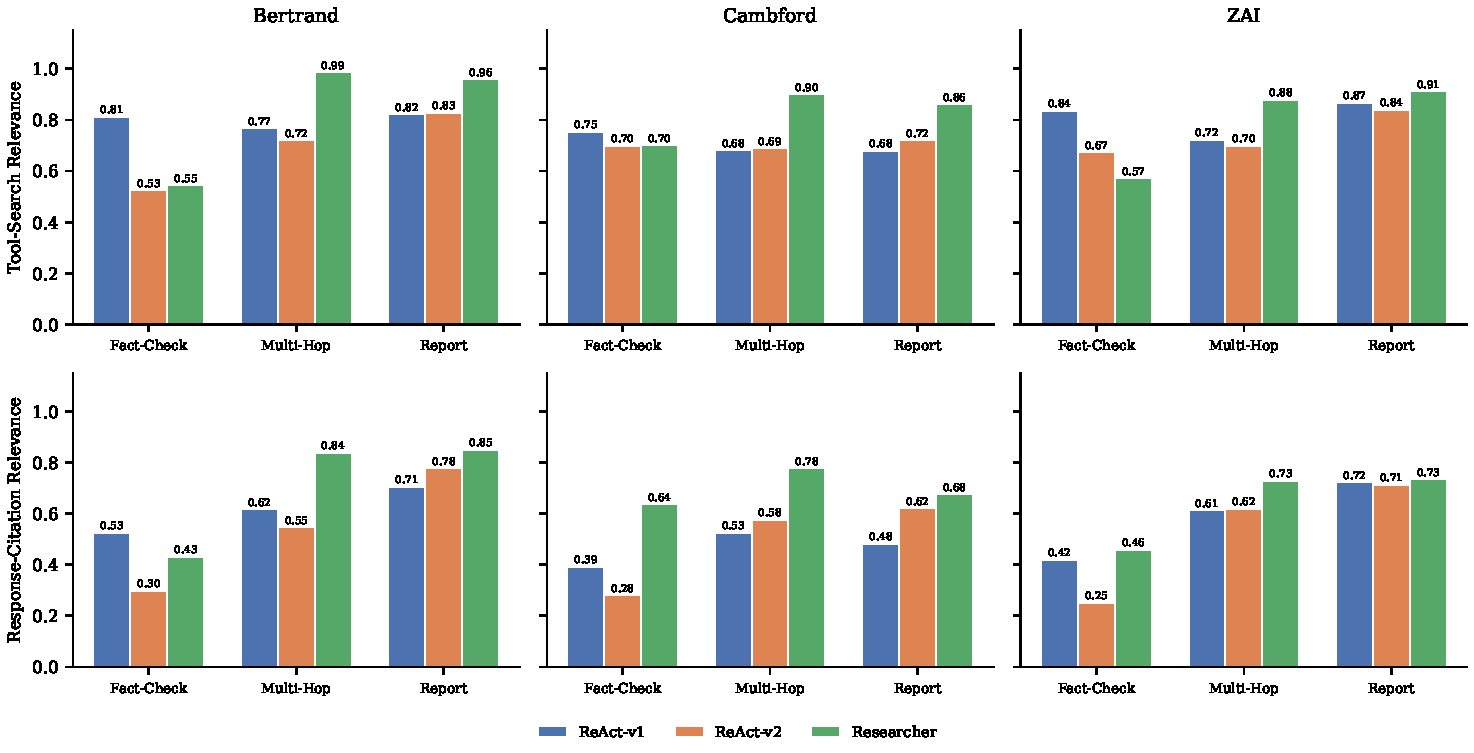
\includegraphics[width=\linewidth]{figures/citation_decomp_by_query_type.pdf}
\caption{Citation decomposition (tool-search relevance and response-citation relevance) by query type. Top row: tool-search relevance; bottom row: response-citation relevance. The performance gap between agents is most visible on comprehensive report queries, where \textsc{Researcher}'s broader retrieval strategy produces higher relevance across both sub-metrics.}
\label{fig:citation_decomp_by_query_type}
\end{figure}

\noindent On targeted artifact search queries, which require locating a single artifact, all three agents achieve their highest assertion scores and the inter-agent gap is narrow. This confirms that when evidence is concentrated in a single entity, even a minimal reactive loop suffices. On multi-hop reasoning queries, assertion scores drop across the board as agents must connect information across multiple artifacts; here \textsc{ReAct-v1}'s detailed worked examples help it maintain higher per-assertion accuracy than \textsc{Researcher}, whose broader retrieval introduces noise. On comprehensive report queries, \textsc{Researcher}'s planning stage provides the clearest advantage in citation quality: its dependency-chain decomposition ensures that multiple source types are systematically retrieved and cited, while the reactive agents struggle to organize comprehensive responses from ad-hoc retrieval sequences.

\textcolor{blue}{\textbf{Post-hoc distribution audit.} To sanity-check that the generator-declared category labels reflect the actual surface form of the queries, we ran a keyword-based audit on all 380 assertions from the \textsc{ReAct-v1}\,$\times$\,Bertrand run. The observed distribution ($\sim$31\% email-anchored, $\sim$20\% file-anchored, $\sim$21\% explicitly cross-source, $\sim$5\% meeting, $\sim$1\% chat, remainder untagged) approximately matches the generator-declared split and confirms that cross-source queries are well represented. This is an automated lexical audit, not a human validation study; a full inter-annotator reliability study on the gold assertions is an open task left for future work.}

\subsubsection{Cost--Effectiveness Trade-off}
\label{sec:cost-tradeoff}

The results reveal a clear cost-effectiveness frontier. \textsc{Researcher} achieves the highest pass rate (35.5\%) and citation quality (0.711) but consumes $5.2\times$ more prompt tokens (92{,}280 vs.\ 17{,}778) than~\textsc{ReAct-v1}. For deployments where retrieval completeness and citation traceability are the primary objectives---legal research, compliance auditing, or due-diligence workflows---this overhead may be justified. For token-sensitive applications or scenarios with dense, recent evidence, \textsc{ReAct-v1} provides 32.3\% pass rate at roughly one-fifth the prompt-token cost with higher factual precision (assertion 0.638 vs.\ 0.557).

\textsc{ReAct-v2} does not occupy a Pareto-optimal point on this frontier: it matches \textsc{ReAct-v1} on tool-call count (1.70) but lags on all quality metrics. This finding suggests that prompt compression is costly in the absence of compensating architectural changes---a concise prompt is not equivalent to an equally effective one. \textcolor{blue}{The \textsc{ReAct-v3} ablation reshapes this frontier: at 0.352 aggregate pass rate, 0.751 composite citation, and \$1.14--\$1.19 per 100 cases, it Pareto-dominates \textsc{ReAct-v1} (same architecture, larger model) and \textsc{Researcher} (same model, added planning) on dollar cost while matching their quality. The practical implication is that a verbose, worked-example prompt on a small model is the most cost-effective configuration we measured.}

\noindent\textbf{\textcolor{blue}{Dollar-cost breakdown.}} \textcolor{blue}{Table~\ref{tab:cost_breakdown} converts the logged per-case prompt and completion token counts to Azure list prices (GPT-4o: \$2.50 / \$10.00 per 1M input / output tokens; GPT-4o-mini: \$0.15 / \$0.60 per 1M). The judge column is the amortised per-case cost of the four judge calls (per-assertion correctness check, tool-search relevance, response-citation quality, and side-by-side comparison) under the same list prices, averaged over the per-tenant case count. The resulting frontier is dominated by \textsc{ReAct-v3}: it matches \textsc{Researcher}'s pass rate at \$1.92--\$2.30 per 162--201-case tenant run versus \$3.15--\$3.91 for \textsc{Researcher}, and at roughly one-fifth the cost of \textsc{ReAct-v1}. \textsc{ReAct-v2} remains Pareto-dominated: it is cheaper than \textsc{ReAct-v1} in dollar terms but delivers materially lower pass rates.}

\textcolor{blue}{
\begin{table}[h]
\centering
\caption{Dollar-cost breakdown per tenant run, derived from logged token counts at Azure list prices. \emph{Agent \$}: cost of the agent loop. \emph{Judge \$}: amortised cost of the four GPT-4o judge calls. \emph{Total \$}: sum. \emph{\$/100}: cost per 100 evaluation cases.}
\label{tab:cost_breakdown}
\small
\begin{tabular}{llrrrr}
\toprule
\textbf{Tenant} & \textbf{Agent} & \textbf{Agent \$} & \textbf{Judge \$} & \textbf{Total \$} & \textbf{\$/100} \\
\midrule
\multirow{4}{*}{Bertrand}
  & \textsc{ReAct-v1}  &  9.50 & 1.16 & 10.66 & 6.58 \\
  & \textsc{ReAct-v2}  &  8.00 & 1.17 &  9.17 & 5.66 \\
  & \textsc{ReAct-v3}  &  0.78 & 1.14 &  1.92 & 1.19 \\
  & \textsc{Researcher} & 1.99 & 1.16 &  3.15 & 1.94 \\
\midrule
\multirow{4}{*}{Cambford}
  & \textsc{ReAct-v1}  &  7.97 & 1.27 &  9.24 & 5.70 \\
  & \textsc{ReAct-v2}  &  7.64 & 1.26 &  8.90 & 5.49 \\
  & \textsc{ReAct-v3}  &  0.61 & 1.26 &  1.87 & 1.15 \\
  & \textsc{Researcher} & 1.95 & 1.26 &  3.21 & 1.98 \\
\midrule
\multirow{4}{*}{ZAI}
  & \textsc{ReAct-v1}  & 11.24 & 1.37 & 12.61 & 6.27 \\
  & \textsc{ReAct-v2}  &  9.12 & 1.38 & 10.50 & 5.22 \\
  & \textsc{ReAct-v3}  &  0.93 & 1.37 &  2.30 & 1.14 \\
  & \textsc{Researcher} & 2.53 & 1.38 &  3.91 & 1.95 \\
\bottomrule
\end{tabular}
\end{table}
}

\begin{figure}[h]
\centering
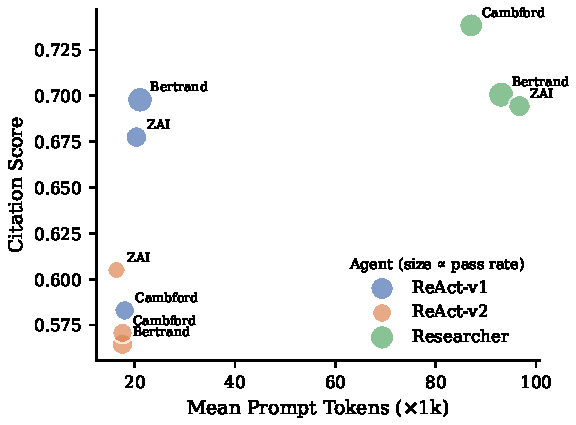
\includegraphics[width=0.7\linewidth]{figures/cost_quality_frontier.pdf}
\caption{Cost--quality frontier: mean prompt tokens vs.\ citation score. Marker size is proportional to pass rate. \textsc{Researcher} achieves the highest citation quality at $5.2\times$ the token cost of the reactive agents; \textsc{ReAct-v2} does not occupy a Pareto-optimal point.}
\label{fig:cost_frontier}
\end{figure}

\subsection{\textcolor{blue}{Threats to Validity}}
\label{sec:threats}
\textcolor{blue}{\textbf{Single-judge dependence.} All reported quality metrics are produced by a GPT-4o judge. To test robustness against judge-model choice, we attempted a replication with GLM-4.7-FlashX as an alternative judge; however, the GLM response formatting diverged sufficiently from our parser's expected schema that the automatically extracted pass rates were systematically deflated to 1--2\% across all agents, which we attribute to parse failures rather than to model disagreement. We therefore do not report cross-model judge numbers, and flag cross-judge robustness as an open validation item. The agent-level rankings reported here should be interpreted as conditional on a single-judge (GPT-4o) protocol.}
